\documentclass{article}
\usepackage{times}
\usepackage{ijcai16}
\usepackage{times}
\usepackage{graphicx}
\usepackage{amsmath}
\usepackage{amsthm, amssymb}
\usepackage{enumerate}
\usepackage{fullpage}
\usepackage{hyperref}
\usepackage{soul}
\usepackage{xcolor}
\usepackage{float}
\usepackage{comment}
\restylefloat{table}
\usepackage{listings}
\usepackage{color} %red, green, blue, yellow, cyan, magenta, black, white
\definecolor{mygreen}{RGB}{28,172,0} % color values Red, Green, Blue
\definecolor{mylilas}{RGB}{170,55,241}
\usepackage{fancybox}
\usepackage{framed}
\usepackage{mathrsfs}
\usepackage{url}
\usepackage{paralist}
\usepackage{booktabs}

\hypersetup{breaklinks=true}
\urlstyle{same}


\graphicspath{{Pictures/}}

\begin{document}
\title{Data Mining Academic Emails to Model Employee Behaviors and Analyze Organizational Structure}
\author{IJCAI-16 Submission 2354}
\maketitle

\begin{abstract}
Email correspondence has become the predominant method of communication for businesses.  If not for the inherent privacy concerns, this electronically searchable data could be used to better understand how employees interact. For example, after the Enron dataset was made available, researchers were able to provide great insight into employee behaviors based on the available data despite the many challenges with that dataset.  The work in this paper demonstrates the application of a suite of methods to an appropriately anonymized email dataset created from volunteers' email metadata.  This new dataset, from an internal email server, is first used to validate machine learning and feature extraction algorithms and then to generate insight into the interactions within the center.  Based solely on email metadata, a random forest approach modeled behavior patterns and accurately classified employees by job title.  The algorithm performed very well not only on participants in the study but also on other members of the center who were connected to participants through email.  Furthermore, the data revealed relationships not present in the formal operating structure.  The result is a much fuller understanding of the center's internal structure than can be found in the official organization chart.
\end{abstract}

\section{Introduction}
A reorganization of a business can be very costly and has great effects once implemented, either for better or for worse.  While this official hierarchy is important, there is an equally important organic organization of any business, which may or may not be reflected in the official organization chart.  Understanding this unofficial structure is important, but due to its informal nature, it can be difficult to determine.  One massive source of electronically searchable information that could be used to better understand this hidden structure is the business's emails.  However, privacy concerns inhibit most research thrusts into email analysis.  

The study presented in this paper collected an appropriately anonymized email metadata dataset to demonstrate to what extent this metadata can be used to determine this organic organizational chart.  Furthermore, this research measured how well this organic organizational chart matches the official organizational chart.  The study utilized email metadata from 37 voluntary participants.  This metadata is used not only to analyze the voluntary participants, but also to see to what extent the non-participant members of the organization can be characterized.

The 98 features used in this study can be grouped into two common areas in email analytics: traffic-based and social-based. Using random forests, these features are used to predict each employee's job title.  The ability to accurately determine job title using as few as three features is demonstrated.  Finally, a comparison between relationships displayed in the data with the formal organizational chart is presented.  

This paper continues by discussing the related works in Section~\ref{Related Works}.  Section~\ref{Data Collection} describes the process of data collection and some statistics of the dataset.  The features extracted from the data are described in Section~\ref{Features}, and the methods investigated using these features are covered in Section~\ref{Analysis}.  The results of the analysis are presented in Section~\ref{Results}.  Section~\ref{Conclusions} concludes the paper and presents opportunities for future work.  

\section{Related Works} \label{Related Works}

Email is a pervasive medium for communication in modern society\textemdash{}particularly in the workplace.  In 2015, there were over 2.6 billion email users~\cite{radicati_emails_2015}.  It is projected that by the end of 2019, over one third of the global population will be using email.  In fact, the average business email user sends and receives a total of 112 emails per day.  Corporate email alone accounts for 54.7\% of worldwide email traffic. Retention of large email archives has become common practice with decreasing memory size and cost~\cite{fisher_revisiting_2006}.  Out of 600 employees at a high-tech company, the average employee had 28,660 emails stored in 133 folders which is a significant increase over the past ten years.  This is a considerable amount of untapped information that could be leveraged to characterize employee roles within an organization.

Since the Enron email dataset was released in 2004 \cite{klimt_introducing_2004}, it has been extensively researched on topics including spam classification \cite{gaber_e-mail_2016}, \cite{shams_classifying_2013}; email categorization \cite{he_novel_2014}, \cite{keila_structure_2005}; and recipient prediction \cite{sofershtein_predicting_2015}, \cite{hu_towards_2012}.  However, there are known flaws and discrepancies with even the most recent versions of this dataset\textemdash{}ranging from misspelled email addresses~\cite{nordbo_data_2014} to duplicate emails~\cite{waterman_big_2014}. In one of the most popular forms of the dataset~\cite{shetty_enron_2004}, the database includes 253,735 emails sent as ``CC'' and  253,713 emails sent as ``BCC''.  Further inspection reveals that emails sent as one type or the other were almost always mistakenly recorded as both.

The existing literature on analyzing social email behavior is mainly divided into two categories: traffic-based and social-based~\cite{tang_email_2013}.  Traffic-based methods calculate statistics based only on email patterns. Social-based methods represent the email communications as a social graph and then extract information from this model using graph-based algorithms.

Using features extracted from email metadata,~\cite{yelupula_social_2008} was able to cluster levels of management at Enron. In addition to email traffic statistics, using features such as the presence of different email attachment types and the length of emails was shown to successfully categorize email behavior in~\cite{martin_analyzing_2005}.

Relational ties can be modeled as a graph network where nodes represent people and edges represent email interactions.  This is a useful model because many statistics can be calculated from the layout of a social graph~\cite{wasserman_social_1994}.  A common metric that has been shown to indicate importance in a social graph is betweenness centrality, which comes in several different flavors first developed by~\cite{freeman_set_1977}.  Betweenness centrality is a measure of how many shortest paths in a graph travel over each node.  A node with high betweenness centrality in a social graph has been shown to represent a high degree of influence on other nodes.  As shown in~\cite{tyler_email_2003}, a betweenness centrality algorithm can be used to determine community structures within an organization.  Other successful metrics were used in~\cite{wilson_discovery_2009}, which detected the most important email users within a corporate network without using betweenness as a feature.  The features used in that study were: degree, the number of edges connected to a node; density, the ratio of actual edges to the number of possible edges; and proximity prestige, the ratio of nodes that can reach a node $i$ to the average distance from those nodes to $i$.

Instead of considering only traffic-based or social-based analytics, these can be be used jointly.  An example of this approach~\cite{rowe_automated_2007}, which combined features such as number of emails, response time, cliques, and degree centrality into a ``Social Score'', was used to rank Enron employees.  

\section{Data Collection} \label{Data Collection}

Over the past decade, the Enron dataset has been widely used to study email behaviors because it is one of the only datasets available comprised of real-world corporate emails.  A list of ground truth job titles was compiled by~\cite{shetty_status_2004}.  However, there are known issues with these labels.  Due to difficulties with the Enron dataset, as described in Section~\ref{Related Works}, this study uses a new dataset generated from volunteers in one of the university's centers.  The center divides its employees into six main areas: directors, graduate students, operations, outreach, project management (PM), and research.

Due to the inherant privacy concerns, researchers worked with the Internal Review Board (IRB) to approve a dataset which maintains participants' privacy.  This dataset is meant to be representative of metadata which any company could use without violating the privacy of their employees.  Special care was taken to protect the privacy of those involved in the study.  During the collection process, all subject and body text was hashed, and all email metadata was stored in a database using scripts without any researchers observing any email text. Furthermore, any identifying information has been omitted from this publication.
The following is the metadata provided from each email:
\begin{compactitem}
\item Destination and source email address
\item Email time stamp
\item Subject prefix (e.g., Re:, Fwd:)
\item Hash of subject after removing prefix
\item Hash of body text
\item Length of subject in characters
\item Length of body text in characters
\item Number of attachments
\end{compactitem}

Table~\ref{tab:db_stats} compares statistics between this internal dataset and the Enron corpus.  This internal database is more modern, contains more emails, and covers a longer time period.  However, it is comprised of fewer people than the Enron dataset.

\begin{table}[H]
\centering
\caption{A comparison between the internal dataset and the Enron email corpus.}
\label{tab:db_stats}
\resizebox{0.5\textwidth}{!}{%
\begin{tabular}{@{}lrr@{}}
\toprule
                   & Center          & Enron         \\ \midrule
Time               & 11/2012-11/2015 & 1/2000-9/2002 \\
Distinct Addresses & 32,118          & 75,406        \\
Participants       & 32              & 249           \\
Distinct Emails    & 585,096         & 252,759       \\ \bottomrule
\end{tabular}
}
\end{table}

While the study includes only 37 volunteers, the email metadata from these volunteers identified 32 additional employees of the center.  These additional employees were included in the study when ground truth for their job was available and when they were identified in at least 100 email metadata records.  This provides 69 total employees in the study.

\section{Features} \label{Features}
The study includes 98 features that were extracted from the email data: 67 traffic-based and 31 social-based.  The traffic-based features are those calculated purely from the collected email metadata.  The social features, on the other hand, first model the email patterns in a graphical network and then calculate statistics from this model.  In the following sections, all features from each of the two categories are described. 

\subsection{Traffic-Based Features}
The simplest traffic-based features used include total number of emails, total sent, and total received.  Other features are calculated based on whether recipients were the primary recipient of the email or were copied on the email.  Similarly, the number of emails sent and received as replies or forwards were also used as features.  Features also included the number of unique email address connections, both sent and received,  and the number of unique email subjects, both sent and received.  The average number of recipients on emails sent and received for each participant were calculated.  It was hypothesized that staff members had more external communications while graduate students communicated more within the university.  To investigate this, the number of emails sent and received from within the center and within the university, based on the domain of the email address, were calculated.  

Other useful information collected from emails included the time stamp, the character counts of the subject and body, and the presence of any attachments. From the time stamp, the time of day for each email was available.  The total number of emails sent and received after hours and the number of emails sent and received after hours within the center were also used as metrics.  For this purpose, after hours was defined as between 6pm and 7am EST on weekdays or anytime on weekends.  The mean and variance of the number of characters in the subject and body were calculated.  These metrics were also broken down between emails sent and received.  The number of attachments sent and received were computed as well as the average number of attachments sent and received per email.  Digitally signing an email is a type of attachment.  Additional features were calculated from the total number of signed emails sent and received, unique email addresses with signed emails, and unique subjects from signed emails.

The features above in general involved raw email counts.  To normalize some of the features, metrics were additionally calculated as a percentage. Examples include the percentage of emails that were sent after hours and the percentage of all received emails with unique subjects out of all received emails.

The best traffic-based feature for predicting employee status was the number of unique subjects received.  This is deemed best because it produces the highest information gain in the feature ranker described in Section~\ref{Analysis}.  This number represents the number of distinct conversations in which an individual was involved.  It is intuitive that people who are involved in more conversations are higher in an organization.  This feature is shown in the histogram in Figure~\ref{fig:traffic_ex_hist}.  It is clear from the figure that GradStudents participated in far fewer email conversations than any other group.  Researchers generated more emails on average, but fewer than the Program Managers.  The directors of the center participate in the most email conversations, by far. 
\begin{figure}[H]
    \centering
        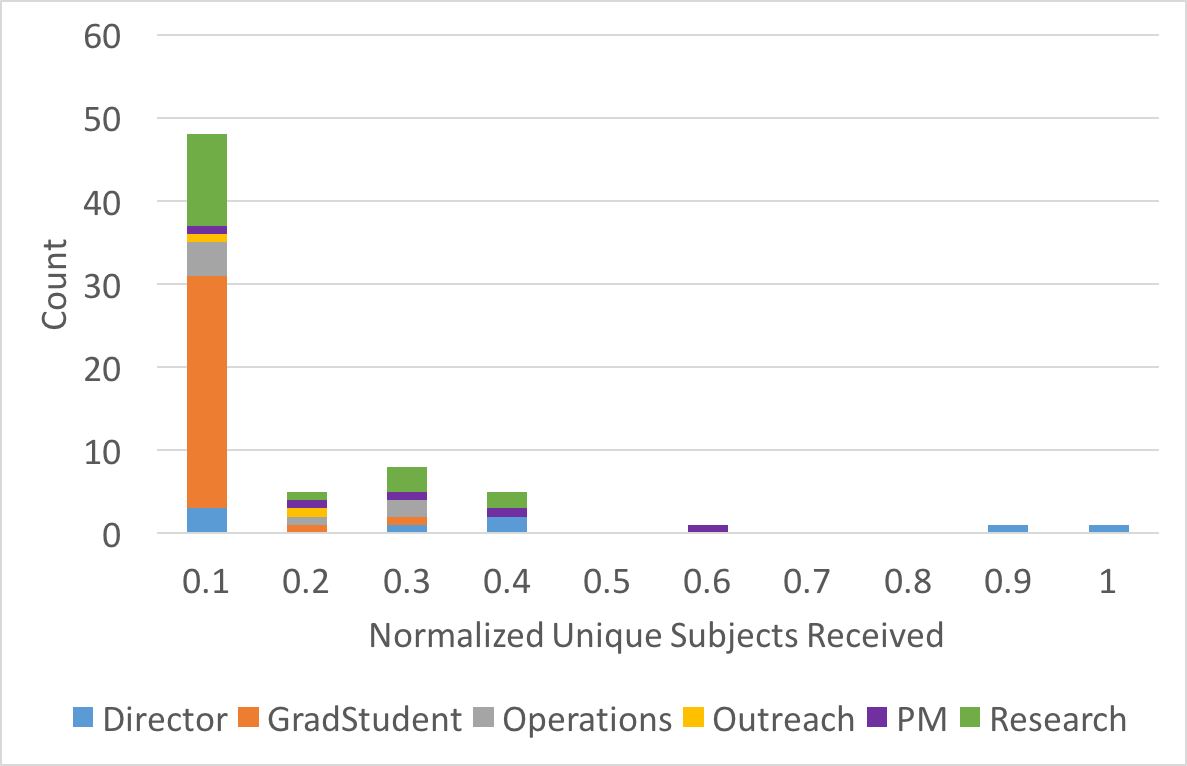
\includegraphics[width=0.5\textwidth]{Unique_subjects_rec_hist}
        \caption{Histogram of unique subjects received by job title.  The feature value for this plot has been normalized so that all values fall between 0 and 1.  Note that by using different thresholds, meaningful splits in the data can be made.  For example, all but two graduate students have a value less than $0.1$.}
        \label{fig:traffic_ex_hist}
\end{figure}

The second best traffic feature was the number of signed emails received.  Signed emails usually signal sensitive information.  Only certain groups within the center deal with this type of information, therefore it is understandable that this feature could help divide the subjects by title.  Finally, the third best traffic feature was the number of emails received as forwards.  Typically, those higher in the chain of command are forwarded emails where graduate students and lower-level employees are more likely to receive either replies or emails sent directly to them.  Notice that there are intuitive explanations behind all of the features selected by the ranker.


\subsection{Social Network Features}
In addition to tracking metadata statistics, features are also derived from modeling the emails as a social network.  A social network is composed of nodes, which represent people, and edges, which represent the emails between people.  For this analysis, two different graphs were generated.  In the full graph, an edge exists between any two individuals that exchanged at least one email.  A second graph only produces an edge between two nodes if at least 10 emails were exchanged.  A representation of the full graph is shown as an adjancency matrix in Figure~\ref{fig:adj_matrix}.  Each of the two axes represent the employees of the center.  The color at each coordinate indicates how much communication existed between the two employees.  Some employees never exchanged any emails, while others exchanged many.

\begin{figure}[H]
    \centering
        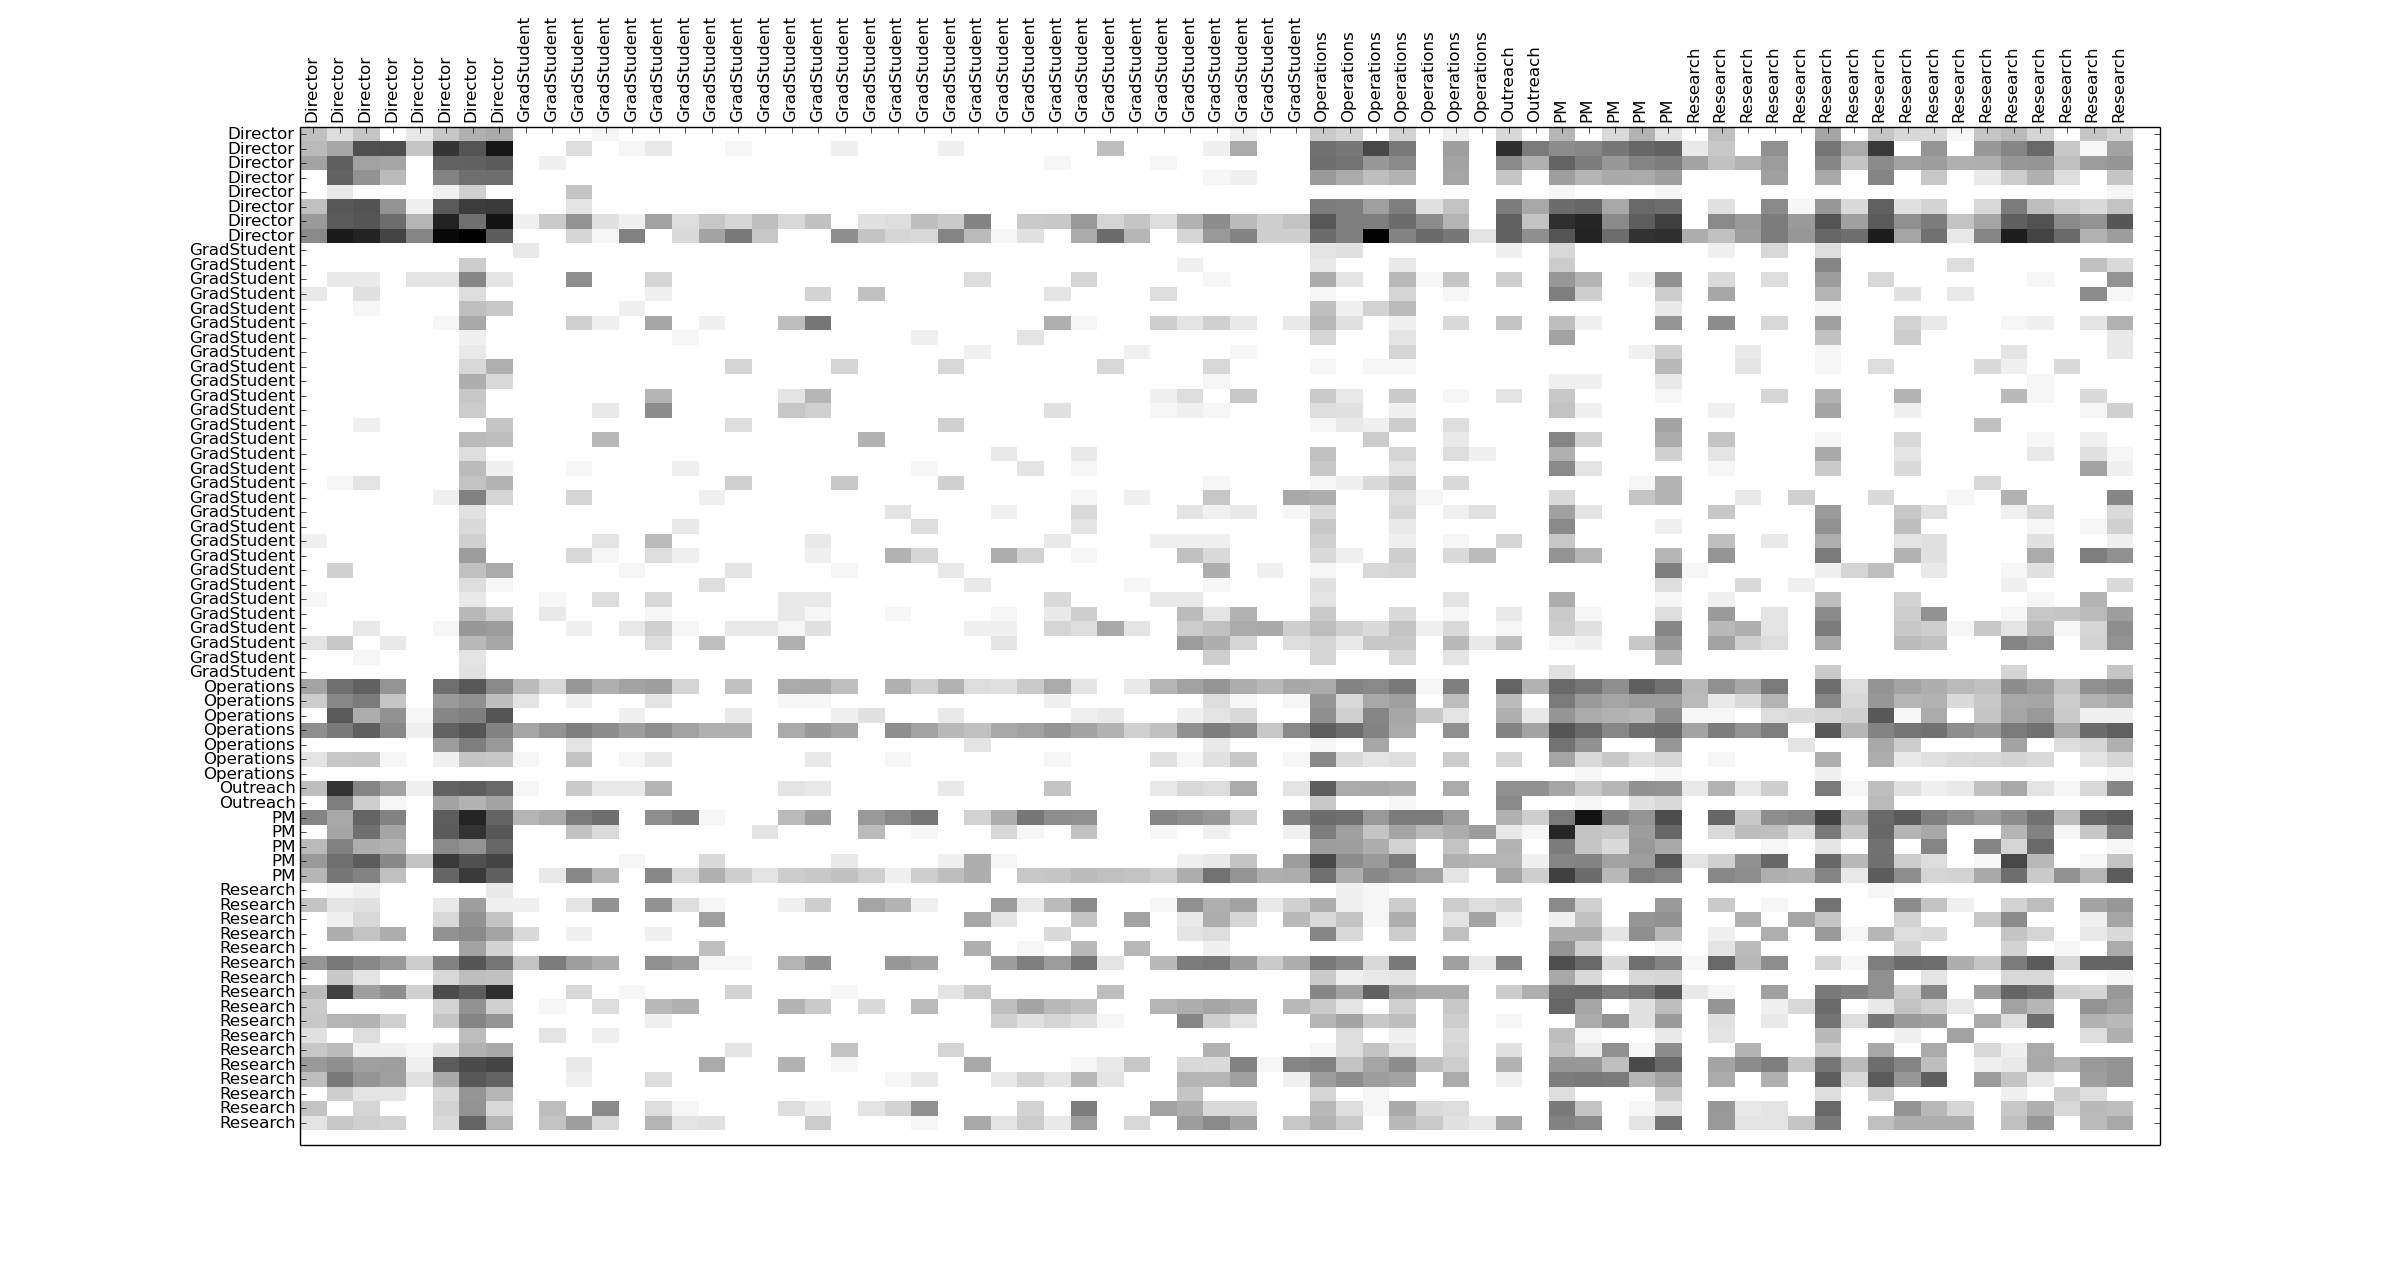
\includegraphics[width=0.5\textwidth]{adj_matrix}
        \caption{The adjacency matrix representing the social connections of the center.  This graph is very well connected with just one component.  Nonetheless, there are groups who never exchanged a single email.}
        \label{fig:adj_matrix}
\end{figure}

With this representation, several statistics can be calculated about the people in the graph.  The average neighbor degree was calculated for both the partial and the full graph.  The degree of a node $i$ is the number of other nodes connected to node $i$.  Therefore for a node $i$, this metric averages the degree of each node in the neighborhood of $i$, that is all nodes connected to $i$.  Mathematically, this is:
\begin{equation}
k_{\text{avg},i} = \frac{1}{|N(i)|}\sum_{j \in N(i)}k_j
\end{equation}
where $N(i)$ are the neighbors of node $i$ and $k_j$ is the degree of node $j$.
The distances between nodes were also used to generate some features.  The average shortest path metric calculates the length of the shortest paths between node $i$ and all other nodes in the graph $G$, and it returns the average of these path lengths.  Similarly, the maximum shortest path length, or eccentricity, was used as a feature in the learning algorithm.  

Some of the social features were based on existing graph theory concepts and algorithms. If a subgraph of a graph $G$ is maximally connected, that is all nodes are connected directly to each other, then this is called a clique.  The number of cliques to which a node belongs was used as a feature.  The hubs and authorities of each node in both graphs were calculated.  The terms hubs and authorities come from the Hyperlink-Induced Topic Search (HITS algorithm) developed by~\cite{kleinberg_hubs_1999}.  This algorithm was originally designed to rate web pages, but has since been applied to social networks. A node's authority is just that\textemdash{}a measure of its importance over other nodes.  A node's hub score is a measure of how well-connected it is to other nodes.  The histogram of hub values in the full graph broken down by class is shown in Figure~\ref{fig:social_ex_hist}.  
\begin{figure}[H]
    \centering
        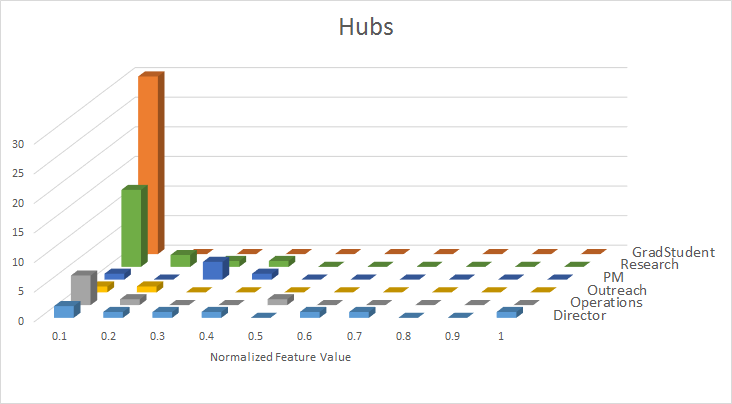
\includegraphics[width=0.5\textwidth]{Hubs_hist}
        \caption{Histogram of hubs from social graph by job title.  Note that directors on average have the highest hub score and graduate students have the lowest.  In fact, three out of eight directors can be identified by filtering samples on full graph hubs values $>0.6$. }
        \label{fig:social_ex_hist}
\end{figure}

Another algorithm used to generate features was the pagerank algorithm, developed by Google 
\cite{page_pagerank_1999} also to rank webpages for search results.  The assumption is that the most important webpages will be linked to frequently by other pages.  Therefore, the ranking is determined by estimating the quality and quantity of links to a node.  The square clustering coefficient for each node was used as a feature. Say there exists a node $i$ with neighbors $j$ and $k$. This metric, developed by~\cite{lind_cycles_2005}, measures the probability that $j$ and $k$ are also neighbors to a fourth node, $l$.  The higher the clustering coefficient, the more connected the node is within its neighborhood.  The triangle clustering coefficient was also used as a metric.  This value, developed by~\cite{saramaki_generalizations_2007}, is the same as the square clustering coefficient but instead determines the probability of connected triangles involving each node.

The majority of the social-based features were centrality measures.  This includes closeness centrality, betweenness centrality, degree centrality~\cite{borgatti2011analyzing}, current flow closeness centrality, current flow betweenness centrality~\cite{brandes2005centrality}, communicability centrality, communicability betweenness centrality~\cite{estrada2008communicability}, and load centrality~\cite{newman2001scientific}.

All of these different graph statistics were used as inputs into the random forest algorithm to characterize each node's importance in the social graph.


\section{Analysis} \label{Analysis}

Due to the large number of features and relatively low number of participants, a classification method was carefully chosen to avoid overfitting the data.  While tree based classifiers can be susceptible to overfitting, the random forest is robust to overfitting issues and was therefore chosen for this study.  The java-based software package Weka was used to generate the random forest based on the algorithm described in~\cite{Breiman2001}.

Random forests are an ensemble method of machine learning, comprised of many random trees.  A random tree is a machine learning algorithm that uses training data to learn a series of rules for classification.  These rules are constructed in a hierarchy that visually resembles a tree.  Each decision is based on what rule will maximize the information gained.  An example random tree with depth three (i.e., it has three levels of rules) is shown below in Figure~\ref{fig:ex_tree}.
\begin{figure}[H]
    \centering
        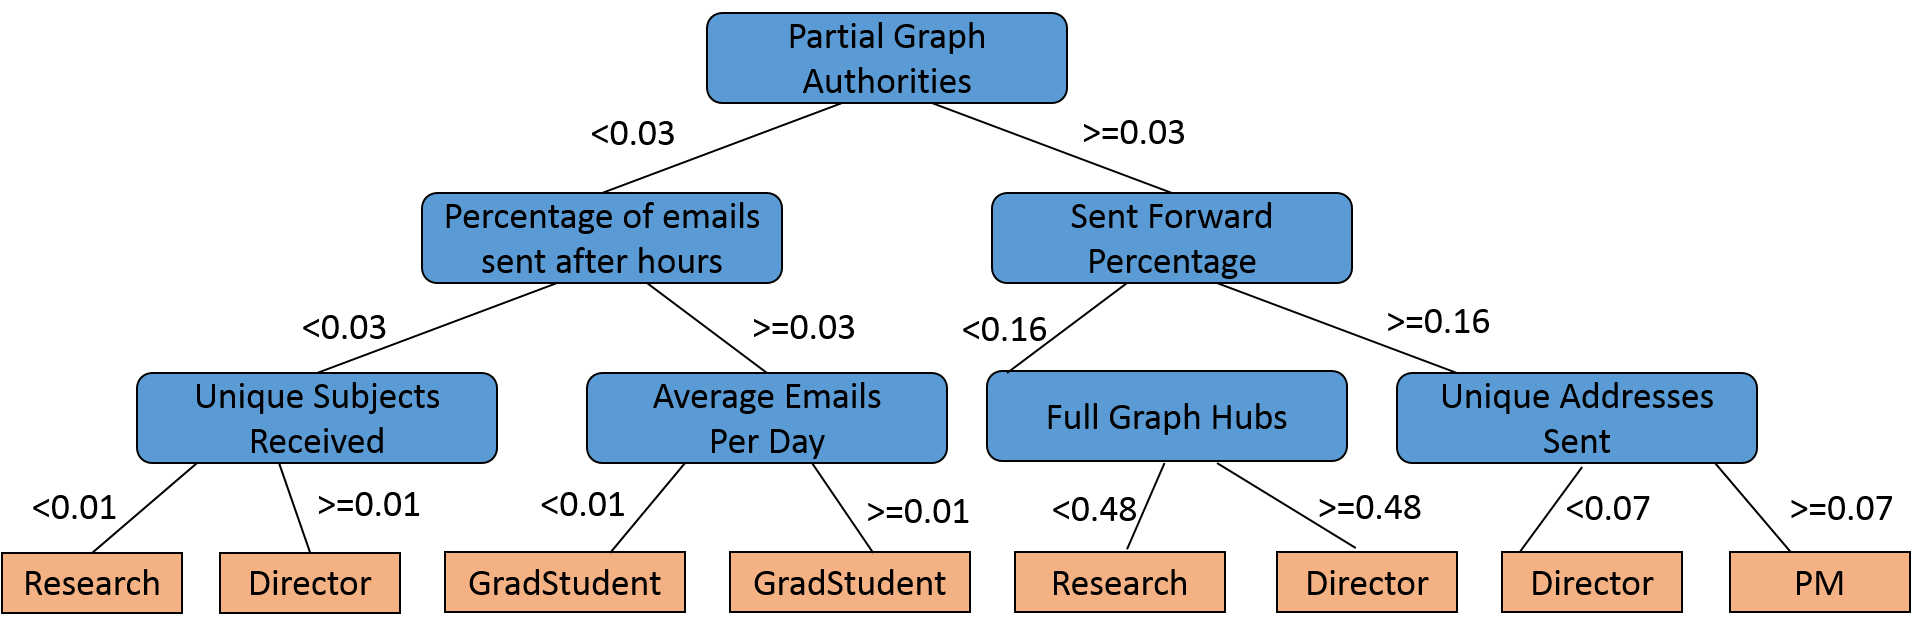
\includegraphics[width=0.5\textwidth]{3_level_tree}
        \caption{Example random tree of depth 3.  This demonstrates how just a few simple rules can be used to find significant class divisions within the data.}
        \label{fig:ex_tree}
\end{figure}

Random forests build many deep random trees with slight random variations.  Individually, these random trees will overfit the data.  However, these many random trees are combined through a process of bootstrap aggregating, or bagging.  In random trials, 750 trees per forest performed optimally for the data.  Therefore, this value was used throughout the analysis.  The bagging process involves each random tree generating a new training data set by sampling observations from the input training set with replacement.  These subsamples are used to build the random trees.  For this analysis, each tree selects $\frac{2N}{3}$ samples to train the trees where $N$ is the number of data points in the overall training set.  Just as the samples were subsampled, so were the features.  Only this subset of features can be used as rules for that tree.  In this implementation, each tree used a subsample of 15 random features.

After all the trees are built, the test data is run through all the random trees in the forest.  Each tree outputs a prediction label for each data point, and the majority vote on each sample is the final predicted label.  Using this random forest model reduces the overall variance and increases the accuracy of the model compared to a single random tree.

Random forests can be difficult to interpret because the ensemble method obscures which features are most meaningful.  An attribute analysis helps to better understand which features are better label predictors.  Since random trees use information gain to dictate splits, information gain was used as the evaluation criteria for the features.  Specifically, each attribute was evaluated by measuring the information gain with respect to the class.  Information gain is calculated as follows for each of the attributes:
\begin{equation}
I(\text{Class}; \text{Attribute}) = H(\text{Class}) - H(\text{Class} | \text{Attribute})
\end{equation} \label{eq:info_gained}
where $I(\text{Class}; \text{Attribute})$ represents the mutual information between the class and the attribute, $H(Class)$ is the entropy of the class variable, and  $H(\text{Class} | \text{Attribute})$ represents the conditional entropy of the Class given the Attribute value.  

Mutual information represents how well knowledge of the attribute informs the prediction of the class.  In this model, both the attribute and the class are treated as random variables.  The entropy of a random variable is a measure of the uncertainty associated with it. After this information gained value was calculated for each feature, they were ranked in order of most important to least.  Table~\ref{tab:ranked_feats} shows the top twenty features from this analysis and the features' corresponding information gain.



\begin{table}[H]
\centering
\caption{Top 20 features ranked by the information gain method.}
\label{tab:ranked_feats}
\resizebox{\columnwidth}{!}{%
\begin{tabular}{@{}lrr@{}}
\toprule
Feature                                      & Type         & Ranker \\ \midrule
Unique subjects received                     & Traffic      & 0.728  \\
Total signed emails received                 & Traffic      & 0.728  \\
Number of emails received as forwards        & Traffic      & 0.719  \\
Full graph hubs                              & Graph        & 0.589  \\
Partial graph communicability centrality     & Graph        & 0.554  \\
PG communicability betweenness centrality    & Graph        & 0.554  \\
Number of emails received as CC              & Traffic      & 0.507  \\
Percentage of emails received as forwards    & Traffic      & 0.503  \\
Partial graph degree centrality              & Graph        & 0.492  \\
Partial graph pagerank                       & Graph        & 0.492  \\
PG current flow closeness centrality         & Graph        & 0.492  \\
Average number of emails received per day    & Traffic      & 0.489  \\
Average total emails per day                 & Traffic      & 0.479  \\
Partial graph average shortest paths         & Graph        & 0.476  \\
Partial graph closeness centrality           & Graph        & 0.476  \\
Unique email addresses from signed emails    & Traffic      & 0.457  \\
Number of emails sent as CC                  & Traffic      & 0.43   \\
Number of emails received as replies         & Traffic      & 0.43   \\
Average emails sent per day                  & Traffic      & 0.404  \\ \bottomrule
\end{tabular}
}
\end{table}

\section{Results} \label{Results}

The results section first shows the algorithm's ability to correctly classify both the study's volunteers and the additional employees identified from the volunteers' emails.  The second part of the results section assumes perfect labeling of the employees and analyzes interactions between employees of different job titles.  The ultimate goal of this research was to determine what additional information can be gained by analyzing the organic organizational chart when compared with the official organizational chart.

\subsection{Classification Results}
Data was split by randomly assigning each email to either the training or testing set with equal probability.  Then, all of the metrics described in Section~\ref{Features} were calculated for both groups separately.  The training data was used as input to the random forest algorithm as described in Section~\ref{Analysis}, and predictions were generated for the test data.  The number of correct and incorrect classifications for each class are shown below in Figure~\ref{fig:result_hist}.  Note that only two predictions were wrong: one person each in research and outreach were misclassified as graduate students.  It is important to note that both  misclassifications are for employees who did not provide their emails for the study.  This means that the classification accuracy for the study participants is 100\%, the percentage of correctly classified inferred employees is 93.75\%, and the overall accuracy of this method using all features is 97.1\%.

\begin{figure}[H]
    \centering
        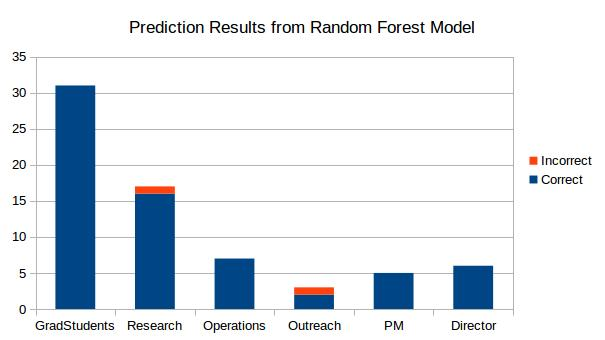
\includegraphics[width=0.5\textwidth]{Prediction_50_50_RF}
        \caption{The Random Forest algorithm was extremely accurate even for very uneven class sizes.  Note that all members of 4 classes were labelled perfectly.  There were only 2 errors out of 69 employees, both of which for employees who did not provide emails for the study.}
        \label{fig:result_hist}
\end{figure}

Note that this method relies on some assumptions.  One is that employees with the same title exhibit similar email behavior.  Overall, based on the success of the algorithm and the distributions of the histograms, this seems to prove true.  Another premise underlying this analysis is that peoples' email behaviors are consistent over time.  This seems to be true as well for the time range in this study.

To determine which features were necessary to the analysis, the algorithm was run several times with a subset of the features.  The first subset used only the top 20 features from Table~\ref{tab:ranked_feats}.  Using only these features resulted in 3 classification errors, or 95.6\% accuracy.  This is only one more error than was found using all 98 features.  For each subsequent run, the least useful feature according to the feature analysis was removed from the input to the system until only one feature remained.  A plot of this analysis is shown below in Figure \ref{fig:feat_analysis}.  Even using just the top thee features resulted in classification accuracy over 80\%.  Therefore, a very good classifier can be built using much fewer features if the features are selected properly.
\begin{figure}[H]
    \centering
        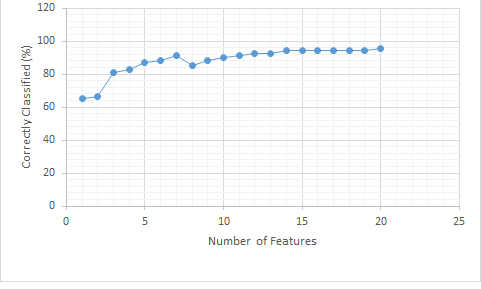
\includegraphics[width=0.5\textwidth]{FeatureAnalysis}
        \caption{Prediction accuracy compared to number of features used for analysis.  Note that the accuracy is still very high, 95.6\%, when only twenty features are used.  The outcome of using only the top twenty features produces three classification errors, only one more than using the full set of 98 features. }
        \label{fig:feat_analysis}
\end{figure}

\subsection{Hierarchy Analysis}
Most of the employees at the center are organized under a director and work with a program manager (unless for example they are a director or program manager).  To generate a metric of how well emails can be used to predict the center's organizational chart, the director and project manager for each applicable employee is predicted from the email metadata. 

The director of each employee is predicted by the algorithm to be the director that the employee communiated with most by email.  Only 57.58\% of the center's employees communicate most frequently with their official director.   This result points to a possible disconnect between the official organization chart and the organic relationships within the center.

To identify each employee's project manager ground truth is selected to be the project that primarily funds the employee.  This time, 72.73\% of graduate students and researchers communicate most frequently with their primary program manager.  The relation between employees to project managers appears to be stronger than that with directors.  Many of the errors in this classification are due to employees who work with multiple project managers.  

\section{Conclusions and Future Work} \label{Conclusions}
This work presents a new dataset, approximately the size of Enron, that was carefully collected from volunteers' emails with particular attention to protect participant privacy.  The new dataset includes accurate labels executed by researchers with intimate knowledge of the center and its employees.  A variety of statistics were calculated from this dataset, and were used in conjunction with a random forest algorithm to automatically classify the center's employees.  Random Forests are shown to be powerful classifiers for this data by predicting employee job titles based on email data with very high accuracy, even for employees for whom only secondhand data is available in the dataset.  Using only 3 features, employees are successfully classified higher than 80\% of the time and are classified over 95\% of the time when 20 features are used.  The email data was also used to show that emails could be used to predict an employee's primary program manager, but had a worse chance of being able to identify the director associated with the employee on the official organizational chart.  This work has shown that it is possible to generate important organizational information from using carefully processed email metadata without compromising the privacy of employees.  Future work in this area will attempt to provide more insight into an organization's organic heirarchy and to apply these algorithms to other datasets to determine the general applicability of the results.

\clearpage
\Urlmuskip=0mu plus 1mu\relax
\bibliographystyle{named}
\bibliography{bib}


\end{document}
